%!TEX root = ../thesis.tex
%*******************************************************************************
%****************************** Second Chapter *********************************
%*******************************************************************************

\chapter{Methods, simulations and data}
\label{ch2:title}


\section{CMIP6 experiment design and data archive}
\label{sec:2.CMIP6}

CMIP, an initiative to compare global climate models, has evolved into a significant international multi-model research activity that has shaped climate science research over the last 20 years \citep{eyringOverviewCoupledModel2016}. CMIP aims to better understand past, present, and future climate change using climate models. An essential part of CMIP is the research community's involvement in designing standardized simulations and output formats that facilitate multi-model analysis. 

As such, models developed worldwide routinely participate in this exercise. According to the CMIP organization literature, the public availability of standardized model output is an important part of CMIP. The broader climate community and users could utilise the data \citep{eyringOverviewCoupledModel2016}. How this project benefits from CMIP is discussed at the end of this section.

\subsection{The DECK experiments}

Since its inception, CMIP has increased complexity and includes more models with diverse complexities and processes \citep{eyringOverviewCoupledModel2016}. Coordination of the project has become more complex, requiring more structure moving forward. CMIP6 proposed a standard set of simulations for all models to tackle this challenge, known as the Diagnostic, Evaluation and Characterization of Klima (DECK). 

According to the CMIP6 overview paper \citep{eyringOverviewCoupledModel2016}, the DECK experiments are designed to provide continuity across past and future phases of CMIP, to be well-established and incorporate simulations that modelling centres perform as part of their own development cycle, and to be relatively independent of the forcings and scientific objectives of a specific phase of CMIP. 

The DECK includes four baseline experiments: a pre-industrial control simulation (\textit{piControl} or \textit{esm-piControl}); a recent historical atmosphere-only Atmospheric Model Intercomparison Project (\textit{amip}); a simulation forced by an abrupt quadrupling of \ce{CO2} (\textit{abrupt-4$\times$CO2}), and finally a simulation forced by a 1\% yr$^{-1}$ \ce{CO2} increase (\textit{1pctCO2}). CMIP6 also suggests a historical transient coupled simulation from 1850 to the present.  The \textit{piControl} experiment serves as the control simulation for the AerChemMIP attribution experiment (see next section), and the historical simulation is used in the same way to provide sea-surface temperatures for \textit{amip}-style attribution experiments in AerChemMIP.

\subsection{The AerChemMIP experiments}

The CMIP6 endorses other projects to evaluate models in specific criteria and goals such as the Aerosol Chemistry Model Intercomparison Project or AerChemMIP \citep{collinsAerChemMIPQuantifyingEffects2017}. The experimental design of AerChemMIP aims to quantify the climate and air quality effects of atmospheric composition change of near-term climate forcings (NTCFs: methane, tropospheric ozone and aerosols, and their precursors). NTCFs especially aerosols were identified in the IPCC AR6 as the main source of uncertainty in the total anthropogenic ERF from 1750 to 2019 \citep[see figure \ref{fig:1.ERF} and][]{forsterEarthEnergyBudget2021}.

The list of AerChemMIP experiments is rather large, being divided into various tiers using different experimental protocols. The experiments from the AerChemMIP that are useful for this research are detailed here. The AerChemMIP proposed historical coupled-ocean experiments which cover the period 1850 to 2014 to attribute aerosols and ozone to climate change over the historical period, i.e. \textit{hist-piNTCF} (aerosol precursors and \ce{O3} precursor emission kept at 1850 level) and \textit{hist-piAer} (aerosol precursor emission kept at 1850 level). 

AerChemMIP also proposes transient historical prescribed SST simulations which use atmosphere-only configurations with prescribed sea surface temperature (SSTs) and sea ice. The use of historical SSTs rather than pre-industrial SSTs eliminate the effects of inconsistent background climate state such as different cloud cover and natural emissions that could affect aerosol and relative species concentrations. This set of historical prescribed SST experiments features more types of chemical species than the historical coupled-ocean experiments mentioned above, making them useful for investigating the effects of oxidant changes on oxidation branching ratio. Experiments that are relevant to \ce{SO2} oxidation include \textit{histSST}, \textit{histSST-piNTCF}, \textit{histSST-piAer}, \textit{histSST-piO3} and \textit{histSST-piCH4}. The suffix -piX denotes that the emission of X species is fixed at the 1850 level.


\subsection{Use cases of CMIP6 and its endorsed MIPs data for this research}

This research, which focuses on \ce{SO2} oxidation, benefits from the existing CMIP and AerChemMIP datasets in the following ways. CMIP \textit{historical} and AerChemMIP historical coupled-ocean experiments could be used to investigate the evolution of \ce{SO2} emission, budget, oxidation branching ratio and their effects on the climate in the historical period. The transient historical prescribed SST simulations are useful for investigating the effects of oxidant changes on sulfate aerosol size distribution and cloud properties.  For the purpose of this work which investigates the atmospheric composition of the atmosphere, the prescribed SST simulations which have a wider range of experiments are more versatile and were employed.



\section{CMIP6 and AerChemMIP experiment design}

This research focuses on \ce{SO2} oxidation and aerosol formation and utilizes data from the AerChemMIP transient historical atmosphere-only prescribed SST simulations \citep{collinsAerChemMIPQuantifyingEffects2017}. These simulations were designed to calculate transient ERFs that drive climate change.  While the simulations were not precisely designed for the purpose of this research, their configurations and emissions align well this research purpose.


Table \ref{tab:2.exps} shows the simulation configurations with all historical transient experiments from AerChemMIP that experiments cover the period between 1850 and 2014. "AOGCM" means atmosphere-ocean coupled simulation. "AGCM" means atmosphere-only simulation. The "AER" suffix means the models should at least calculate tropospheric aerosol driven by emission fluxes. The "CHEM$^\text{S}$" suffix means at least stratospheric chemistry is required; "CHEM$^\text{T}$" means at least tropospheric chemistry is required. "Hist" means the concentration or emission should evolve as for the CMIP historical simulation. "1850" means the concentrations or emissions should be fixed to the year 1850. 

\begin{table}
   \caption[AerChemMIP experiments related to this work]{A summary of AerChemMIP experiments related to this work.}
   \label{tab:2.exps}
   \centering
   \begin{tabular}{l p{30mm} l p{18mm} p{18mm} l}
    \toprule
     Experiment ID & Minimum model configuration & \ce{CH4} & Aerosol precursors & \ce{O3} precursors & suite-id \\
    \midrule
     \textit{historical}      & AOGCM AER & Hist & Hist & Hist & u-bc179\\
     \textit{hist-piAer}      & AOGCM AER & Hist & 1850 & Hist & u-bg705\\
     \textit{hist-piNTCF}     & AOGCM AER & Hist & 1850 & 1850 & u-bg946\\
     \textit{histSST}         & AGCM AER & Hist & Hist & Hist & u-bh626\\
     \textit{histSST-piAer}   & AGCM AER & Hist & 1850 & Hist & u-bi541\\
     \textit{histSST-piO3}    & AGCM CHEM$^{\text{T}}$ & Hist & Hist & 1850 & u-bl670\\
     \textit{histSST-piCH4}   & AGCM CHEM$^{\text{T/S}}$ & 1850 & Hist & Hist & u-bl551\\
     \textit{histSST-piNTCF}  & AGCM AER & Hist & 1850 & 1850 & u-bl277\\
     \bottomrule
   \end{tabular}
\end{table}



\change[inline]{comment on how there is another set of simulations but was not run by UKESM1 hist-aer etc which is a limitation for this work.}




\section{Aerosol effective radiative forcing calculation}
\label{sec:ch2:erf}

Aerosol affects the climate directly via scattering and indirectly by altering the thermal structure of the atmosphere and hence cloud thermodynamics (aerosol direct effect or aerosol-radiation interaction), and via microphysical effects such as increasing the number of condensation nuclei and and decreasing the effective radii of cloud droplets, referred to as the aerosol cloud albedo effect and the cloud lifetime effect \citep{twomeyInfluencePollutionShortwave1977}.
%(Twomey, 1974; Albrecht, 1989; Pincus and Baker, 1994). 

The ERF is calculated from the difference in the net top-of-atmosphere radiative flux ($\Delta F$) between the perturbed simulation (e.g. \textit{piAer}) and \textit{histSST} simulation as  $\text{ERF} = \Delta F$

To understand the contributions of various processes to the overall effective radiative forcing (ERF) we can separate the ERF that is due to direct radiative forcing from that due to the effects of clouds and aerosol instantaneous radiative effects. Following the method of \citet{ghanTechnicalNoteEstimating2013}, the contribution of the aerosol-radiation interactions to the ERF can be distinguished from that of the aerosol–cloud interactions by using a "double-call" method.

% describe double call method
In the "double-call" method, radiative flux diagnostics are calculated first for all-sky and then again ignoring the scattering and absorption of solar radiation by the aerosol. For each call, the model calculates the shortwave radiative flux at the top of the atmosphere (TOA) and a diagnostic TOA flux with with cloud neglected. The first call yields all-sky TOA shortwave flux, $F$, and clear sky, i.e. "cs", flux, $F_{\text{cs}}$. The second call, the aerosol-free or clean-sky, yields clean sky TOA shortwave flux, $F_{\text{clean}}$, and clean-and-clear TOA shortwave flux, $F_{\text{cs,clean}}$.

This way, direct radiative forcing from aerosol could be calculated by subtracting clean sky flux from all-sky flux, $\Delta (F - F_{\text{clean}})$. Cloud radiative forcing is then calculated from the cloudy part of the sky by subtracting clean and clear sky flux with clean sky flux, $\Delta (F_{\text{clean}} - F_{\text{cs,clean}})$. Finally, the surface albedo and greenhouse gas effects are calculated from the clean and clear sky flux, $\Delta F_{\text{cs,clean}}$. This could be summarised as follows.
\begin{equation}[] 
\label{eq:erf}
\begin{split}
\text{ERF} &=  \Delta(F-F_{\text{clean}}) + \Delta F_{\text{cs,clean}} + \Delta ({F_{\text{clean}}-F_{\text{cs,clean}}}) \\
 & = \text{AerosolIRF} + \text{ERF}_{\text{cs,clean}}+\Delta \text{CRE}'
\end{split}
\end{equation}

We also note that the definition of transient ERF used here differs from the usual definition of effective radiative forcing (ERF) where the SSTs are specified to be fixed repeating climatology \citep{eyringOverviewCoupledModel2016}. In contrast, The SSTs in the experiments are from prescribed historical SSTs, with all emissions set as historical. This work defines transient ERF as a global average of the difference in the top-of-atmosphere radiative flux. The average is calculated as a moving decadal mean.   




\section{UKESM1 model}  
\label{sec:1.ukesm1}

\subsection{Model description}
UKESM1 is a coupled atmosphere-ocean climate model, based on the Global Coupled model version 3.1 \citep[HadGEM3-GC3.1;][]{kuhlbrodtLowResolutionVersionHadGEM32018, brownUnifiedModelingPrediction2012}, Nucleus for European Modelling of the Ocean (NEMO) model \citep{storkeyUKGlobalOcean2018}, the Los Alamos Sea Ice (CICE) model \citep{ridleySeaIceModel2018} and utilising separate the Join UK Land Environment Simulator (JULES) model for the land surface \citep{bestJointUKLand2011} and the Model of Ecosystem Dynamics, nutrient Utilisation, Sequestration and Acidification (MEDUSA) model to simulate ocean biogeochemistry \citep{yoolMEDUSA2IntermediateComplexity2013}. UKESM1 also features the stratospheric-tropospheric atmospheric chemistry scheme (StratTrop) implemented as part of the United Kingdom Chemistry and Aerosol (UKCA) model \citep{archibaldDescriptionEvaluationUKCA2020}, which is coupled with the aerosol scheme GLOMAP-mode \citep{mulcahyDescriptionEvaluationAerosol2020}. 


%The atmospheric chemistry, aerosol and cloud schemes modelled by the UKCA model that is relevant to the sulfur cycle are briefly described here. 
The emission of DMS from natural sources is taken from the MEDUSA component which calculates the emission using the emission scheme from \citet{lissAirSeaGasExchange1986}. Anthropogenic \ce{SO2} emissions follow \citet{hoeslyHistorical175020142018}, and tropospheric volcanic emissions from continuously degassing volcanoes are prescribed over the historical period \citep{andresTimeaveragedInventorySubaerial1998, dentenerEmissionsPrimaryAerosol2006}.  Note that all anthropogenic \ce{SO2} is emitted at the lowest layer of the model. Oxidation of \ce{SO2} and DMS is treated online via the UKCA module, which includes photolysis, dry and wet deposition and in-cloud chemistry \citep{mulcahyDescriptionEvaluationAerosol2020}. Wet deposition is parameterised using \citet{giannakopoulosValidationIntercomparisonWet1999} scheme, and the dry deposition scheme takes into account the land surface types from the JULES model using a resistance type model from \citet{weselyParameterizationSurfaceResistances1989}. In the UKCA StratTrop, DMS is not deposited at all, while \ce{SO2} and \ce{SO4} are both wet and dry deposited \citep{archibaldDescriptionEvaluationUKCA2020}. Aerosol is treated with a two-moment modal global aerosol microphysics scheme \citep[GLOMAP-mode;][]{mannDescriptionEvaluationGLOMAPmode2010}. 

GLOMAP-mode, a two-moment aerosol scheme, simulates aerosol mass and size independently \citep{mannDescriptionEvaluationGLOMAPmode2010}. This is in contrast to a one-moment scheme, which assumes a linear relationship between aerosol mass and size, and only aerosol mass is predicted. The aerosol-cloud interactions are susceptible to the treatment of precipitation \citep{gettelmanAdvancedTwoMomentBulk2015}. Compared to single-moment cloud microphysics schemes, double-moment schemes have reduced a range of biases in high-resolution climate models \citep{seikiImprovementGlobalCloudSystemResolving2015}. 

\begin{table}
   \caption[Standard configuration for aerosol in GLOMAP-mode]{A summary of standard configuration for aerosol in GLOMAP-mode \citep{mannDescriptionEvaluationGLOMAPmode2010}}
   \label{tab:glomap}
   \centering
   \begin{tabular}{l l}
    \toprule
     Aerosol mode & Size range  \\
    \midrule
     Nucleation mode & $\overline{D} < 10$ nm \\ 
     Aitken mode & $10 < \overline{D} < 100$ nm \\
     Accumulation mode & $100 < \overline{D} < 1000$ nm\\
     Coarse mode & $ \overline{D} > 1000$ nm\\
     \bottomrule
   \end{tabular}
\end{table}


\subsection{Sulfate production rates in UKESM1}
\label{ch2:sec:so4-prod-rate}

The majority of sulfate aerosols are produced in the atmosphere via oxidation. Approximately 5\% of total sulfate production is from primary emissions, which reflects 2.5\% of anthropogenic \ce{SO2} emissions that are assumed to enter the atmosphere as sulfate aerosols. The other 95\% of sulfate aerosol in UKESM1 are produced in two pathways: gas-phase oxidation of \ce{SO2} and OH, producing sulfuric acid, which nucleates into new particles, and aqueous-phase oxidation in cloud droplets. 

Gas-phase oxidation of \ce{SO2 + OH} is a termolecular reaction, Reaction \ref{ch1:eq:so2-oh}, with the parameters for rate constant given in Table \ref{ch4:tab:so2-oh-reaction-consts} a function of the concentration of air, [M], and temperature, T.
\begin{align}
    \dfrac{d[\ce{SO2}]}{dt} =  k_{([M],T)} [\ce{SO2}][\ce{OH}][\ce{M}] \label{ch4:eq:so2-oh-prod}
\end{align}

The rate constant for the termolecular reaction, $k_{([M],T)}$, is given below.
\begin{align}
    k_0 &= k_1 \left(\frac{T}{300}\right)^{\alpha_1} \exp{(-\beta_1/T)} \label{ch4:eq:so2-oh-k0}\\
    k_\infty &= k_2 \left(\frac{T}{300}\right)^{\alpha_2} \exp{(-\beta_2/T)} \label{ch4:eq:so2-oh-k_inf}\\
    k_{([M],T)} &= \left( \frac{k_0[M]}{1+\frac{k_0[M]}{k_\infty}}\right) F_c^{\left\{ 1+\left[ \log_{10} \left( \frac{k_0[M]}{k_\infty}\right) \right]^2 \right\}^{-1}} \label{ch4:eq:so2-oh-k_MT} 
\end{align}

The free radical \ce{HSO3} reacts in a chain of reactions with \ce{O2} and \ce{H2O} to form \ce{H2SO4}.

\begin{table}[]
\centering
    \begin{tabular}{ccccccccc}
    \hline
    Reactants & Products & $F_c$ & $k_1$ & $\alpha_1$ & $\beta_1$ & $k_2$ & $\alpha_2$ & $\beta_2$ \\ \hline
    \ce{SO2 + OH} & \ce{SO3 + HO2} & 0.60 & 3$\times 10^{-31}$ & -3.3 & 0 & 1.5$\times 10^{-12}$ & 0 & 0 \\ \hline
    \end{tabular}
\caption{constants for \ce{SO2 + OH} reaction}
\label{ch4:tab:so2-oh-reaction-consts}
\end{table}

The aqueous-phase reactions in UKESM1 require information about cloud droplets and cloud droplet acidity as acidity determines rates of \ce{SO2 + O3} and \ce{SO2 + H2O2} reactions \citep{seinfeldAtmosphericChemistryPhysics2016}. Once the reaction rates are determined from Equation \ref{ch1:eq:so2-o3}--\ref{ch1:eq:so2-h2o2}, the in-cloud sulfate aerosol production is obtained from
\begin{align}
    \Delta S_{\mathrm{cloud}} = F \cdot \left( \dfrac{d[S(IV)]}{dt}\right) \cdot L \cdot N_a \cdot \frac{1}{\rho_w} \label{ch4:eq:in-cloud-sulfate-prod}
\end{align}
where $F$ is the cloud fraction, $ \dfrac{d[S(IV)]}{dt}$ is the aqueous-phase reaction rate, $L$ is the cloud liquid water content, $N_a$ is the Avogadro's constant, and $\rho_w$ is the density of water. In the model version used in this work, global cloud pH is set to 4.0 where the local \ce{SO2} mixing ratio exceeds 0.5 ppb, or 5.0 if not.


GLOMAP-mode, the aerosol module simulating aerosol processes in UKESM1, treats aerosol number concentration for each aerosol mode separately with interaction such as coagulation and between modes. The aerosol number for each mode is represented by a log-normal distribution with a geometric mean diameter $\bar{D}$ covering the nucleation ($\bar{D} < 10$ \unit{\nano\metre}), Aitken ($10 \leq \bar{D} < 100$ \unit{\nano\metre}), accumulation ($100 \leq \bar{D} < 1000$ \unit{\nano\metre}), and coarse ($\bar{D} \geq 1000$ \unit{\nano\metre}) mode. The mass concentration of each component, including sulfate, sea salt, black carbon, organic carbon and dust in each mode, is also calculated separately. 


% \subsection{Specific ERF}
% \subsection{Adjusted HadCRUT5}
% \subsection{Seasonal mean surface anomaly}


The following sub-section explores the theoretical range of all oxidation pathways due to variations in temperature, cloud droplet pH, and cloud fraction to confirm the modelled observation.

\subsubsection{Theoretical range of \texorpdfstring{\ce{SO2}}{SO2} oxidation reaction rates}

In this section, I quantify the factors that limit sulfate production rates in summer and winter conditions by calculating the rates from equations in UKESM1 using parameter values from observation or model averages. 

The equations describing sulfate production includes Equation \ref{ch4:eq:so2-oh-prod}--\ref{ch4:eq:so2-oh-k_MT} for gas-phase reactions, and Equation \ref{ch1:eq:Henry-eq}--\ref{ch1:eq:aq-conc} and \ref{ch4:eq:in-cloud-sulfate-prod} for aqueous-phase reactions. The parameters needed for the gas-phase reaction include concentration of OH and \ce{SO2}, atmospheric temperature and pressure. Aqueous-phase productions by \ce{O3} and \ce{H2O2} are more complex and require cloud parameters, including cloud fraction, liquid water content and cloud pH, in addition to oxidant concentrations, atmospheric temperature and pressure. 


\begin{figure}
    \centering
    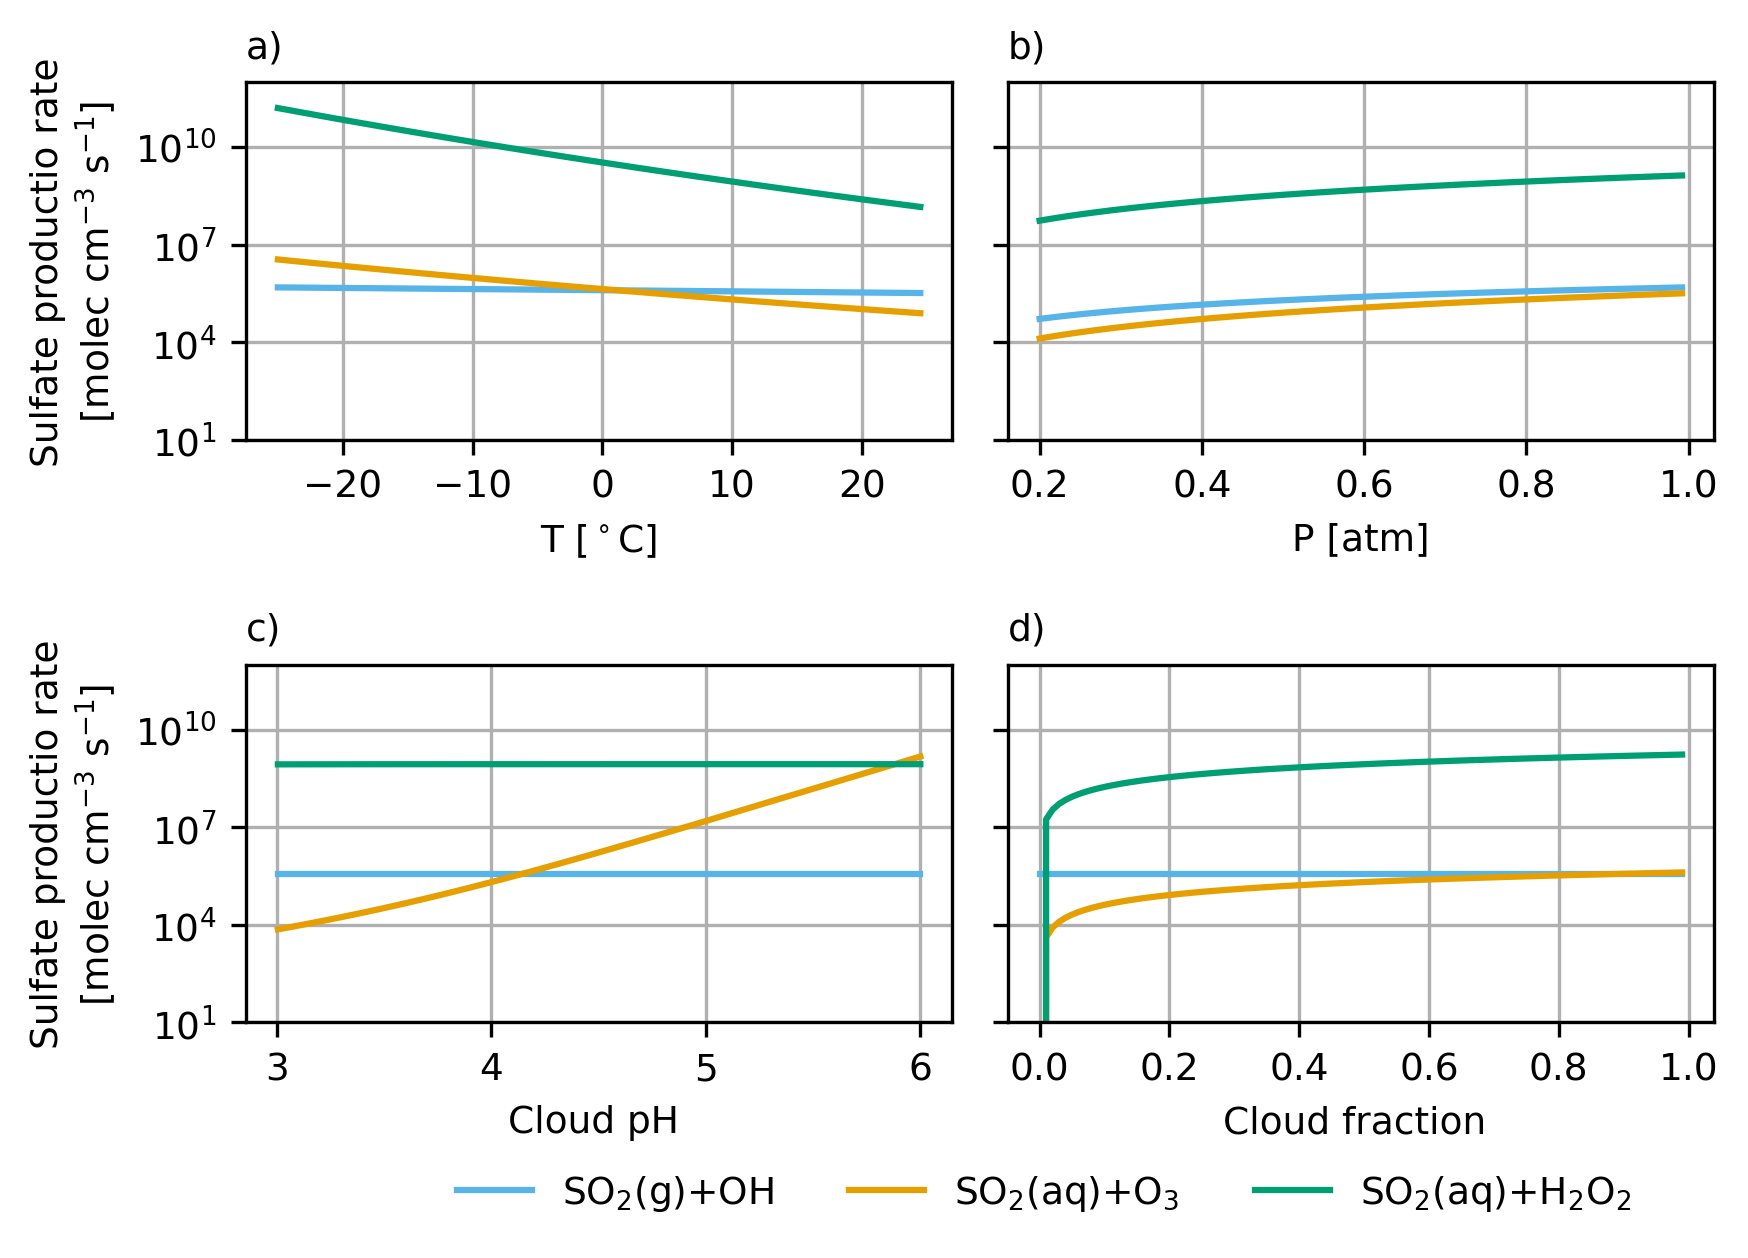
\includegraphics{Chapter4/Figs/oxidation_sensitivity.png}
    \caption[\ce{SO2} oxidation range]{\ce{SO4} production rates for a range of a) atmospheric temperature, b) pressure, c) cloud pH and d) cloud fraction when other parameters are set to average values shown in the first three rows in Table \ref{ch4:tab:sensitivity-test}.}
    \label{fig:ch4:oxidation-sensitivity}
\end{figure}

Changes in sulfate production rates due to temperature, pressure, cloud pH and cloud fraction are shown in Figure \ref{ch4:tab:sensitivity-test}. \ce{SO2 + O3} produces sulfate faster than \ce{SO2 + OH} when the temperature drops below zero \textdegree C, a condition more common in winter and at higher altitudes. Cloud pH strongly influences \ce{SO2 + O3}. \ce{SO2 + O3} oxidation is slower than all other reactions by approximately one order of magnitude except when cloud pH equals 6.0. In this case, \ce{SO2 + O3} reaction rate is the same magnitude as \ce{SO2 + H2O2}. However, this pH is not present in UKESM1 as cloud pH is set to 4.0 or 5.0, depending on the concentration of \ce{SO2}. This thus limits the importance of \ce{SO2 + O3}. Cloud properties do not affect \ce{SO2 + OH} since it is a gas-phase reaction, whereas the aqueous-phase reactions are strongly dependent on cloud fractions, especially when the cloud fraction is below 0.1. 


\begin{table}
\centering
\begin{tabular}{p{1.8cm} p{1cm} p{1.25cm} p{1cm} p{1cm} p{0.8cm} p{1cm} p{1cm} p{1cm} p{1cm}}
\toprule
 & \ce{SO2} [ppb] & OH conc. [cm$^{-3}$] & \ce{O3} [ppb] & \ce{H2O2} [ppb] & pH & T [\textdegree C] & P [atm] & CF & LWC [kg m$^{-3}$] \\ \midrule
Average value & 20.0 & 1.0$\times 10^{6} $ & 40.0 & 2.0 & 4.0 & 10.0 & 0.8 & 0.5 & 0.0002 \\
% Minimum & 5.0 & 1.0$\times 10^{5} $ & 20.0 & 0.2 & 3.0 & -25.0 & 0.2 & 0.01 & 0.0002 \\
% Maximum & 50.0 & 5.0$\times 10^{7} $ & 120.0 & 4.6 & 6.0 & 25.0 & 1.0 & 1.0 & 0.0002 \\ 
\midrule
Summer average & 5.0 & 1.0$\times 10^{6} $ & 60.0 & 2.0 & 4.0 & 15.0 & 0.8 & 0.01 & 0.0002 \\
Summer daytime & 20.0 & 5.0$\times 10^{7} $ & 110.0 & 4.6 & 4.0 & 25.0 & 0.8 & 0.01 & 0.0002 \\
Summer nighttime & 10.0 & 3.0$\times 10^{5} $ & 40.0 & 0.1 & 4.0 & 10.0 & 0.8 & 0.01 & 0.0002 \\ \midrule
Winter average & 50.0 & 5.0$\times 10^{5} $ & 30.0 & 1.0 & 4.0 & 0.0 & 0.8 & 0.5 & 0.0002 \\
Winter daytime & 70.0 & 1.0$\times 10^{6} $ & 55.0 & 2.4 & 4.0 & 5.0 & 0.8 & 0.5 & 0.0002 \\
Winter nighttime & 20.0 & 1.0$\times 10^{5} $ & 20.0 & 0.1 & 4.0 & -5.0 & 0.8 & 0.5 & 0.0002 \\ \midrule
Annual average & 20.0 & 1.0$\times 10^{6} $ & 30.0 & 1.0 & 4.0 & 10.0 & 0.8 & 0.1 & 0.0002 \\
Annual daytime average & 20.0 & 1.0$\times 10^{7} $ & 60.0 & 2.0 & 4.0 & 15.0 & 0.8 & 0.1 & 0.0002 \\
Annual nighttime average & 20.0 & 1.0$\times 10^{5} $ & 20.0 & 0.1 & 4.0 & 5.0 & 0.8 & 0.1 & 0.0002 \\ \midrule
UKESM1 summer & 0.1 & 1.4$\times 10^{6} $ & 37.6 & 0.8 & 4.0 & 10.0 & 0.8 & 0.01 & 0.0002 \\
UKESM1 winter & 0.2 & 1.1$\times 10^{6} $ & 31.3 & 0.7 & 4.0 & 10.0 & 0.8 & 0.5 & 0.0002 \\
UKESM1 annual average & 0.2 & 1.3$\times 10^{6} $ & 34.4 & 0.8 & 4.0 & 10.0 & 0.8 & 0.1 & 0.0002 \\ \bottomrule
\end{tabular}
\caption[Parameters for oxidation rates]{Parameters for oxidation rate. CF is cloud fraction, and LWC is liquid water content. Summer, winter, and annual daytime and nighttime averages are taken from field campaigns with similar characteristics (urban areas) where possible. UKESM1 data are taken from Figure \ref{fig:ch4:seasonal-oxidants}, which are monthly mean values.}
\label{ch4:tab:sensitivity-test}
\end{table}


% Describe the oxidant values from different measurement campaigns
The ranges of the sulfate production rates in summer and winter are calculated using oxidant concentrations from different measurement campaigns listed in Table \ref{ch4:tab:sensitivity-test}. \ce{SO2} concentrations are from an urban area in Beijing, China \citep{linCharacteristicsRecentTrends2012}. OH concentrations are taken from two measurement campaigns to cover nighttime and daytime from an urban site in Birmingham, UK \citep{heardHighLevelsHydroxyl2004, khanNighttimeNO3OH2008}. \ce{H2O2} concentrations are taken from rural measurements in Guangzhou, China \citep{huaAtmosphericHydrogenPeroxide2008}. The cloud pH is set to 4.0 as the aerosol module in UKESM1 uses a cloud pH of 4.0 when the concentration of \ce{SO2} is greater than 0.5 ppb \citep{mannDescriptionEvaluationGLOMAPmode2010}. Pressure, cloud fraction and liquid water content are treated as constants.

\begin{figure}
    \centering
    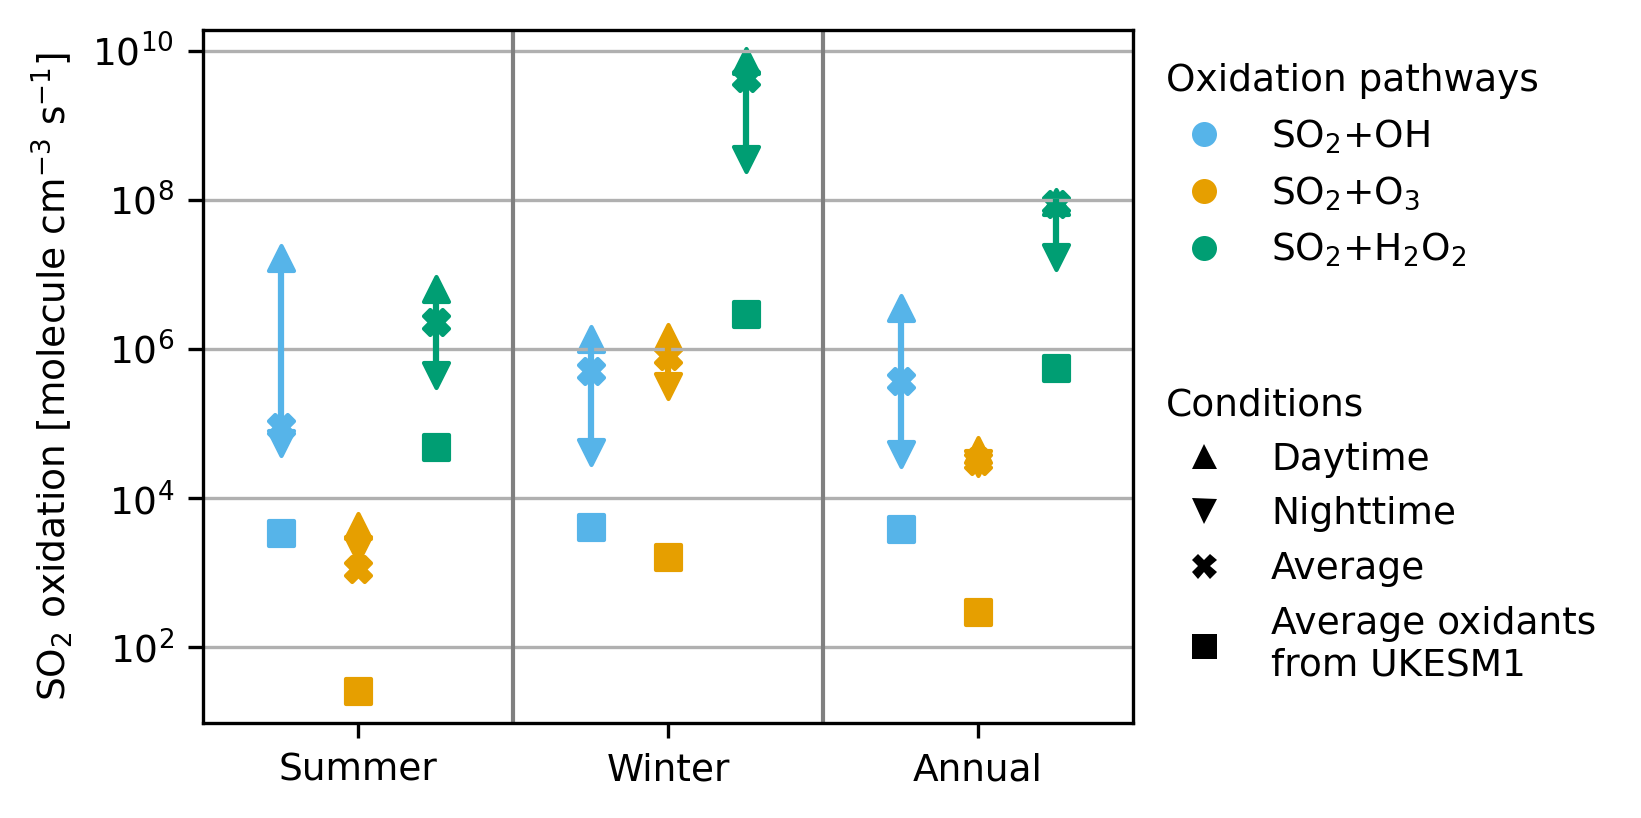
\includegraphics{Chapter4/Figs/theoretical_oxidation.png}
    \caption[\ce{SO4} production rates calculated for summer, winter, and average conditions]{\ce{SO4} production rates calculated for summer, winter, and average conditions as given in Table \ref{ch4:tab:sensitivity-test}.}
    \label{fig:ch4:sensitivity-summary}
\end{figure}

% Explain summer variations for OH
Figure \ref{fig:ch4:oxidation-sensitivity} shows the range of \ce{SO2} oxidation reaction rate in summer and winter using conditions from Table \ref{ch4:tab:sensitivity-test}. \ce{SO2 + OH} is the greatest of all pathways in summer when the temperature and OH concentration are high while the cloud fraction is low. Oxidation by \ce{O3} is the weakest due to low cloud fraction and high temperature. \ce{SO2 + OH} is lower in winter due to lower OH concentration while temperature has negligible effects, as shown in Figure \ref{fig:ch4:oxidation-sensitivity}. 

In contrast, aqueous-phase production by \ce{O3} and \ce{H2O2} increases by two orders of magnitudes in winter compared to summer conditions, placing \ce{SO2 + O3} in the same order of magnitude of \ce{SO2 + OH}. This increase in aqueous-phase production in winter comes from more significant cloud fractions. 


\subsection{Model validation}
\change[inline]{Add model validation}



\section{Aerosol size distribution from log-normal distribution}
\change[inline]{Describe calculation of aerosol size distribution}


\section{Definitions of terms and methods}
\label{sec:2.terms}
The main definitions used in this work relate to the concept of the atmospheric chemical budget. The budget of a trace gas consists of three quantities: its global source, global sink, and atmospheric burden. For the sulfur budget, all masses are represented in the Tg of sulfur, not in the Tg of \ce{SO2}.

\subsubsection{Source / Emission}

The source of a trace gas (Tg yr$^{-1}$) is the sum of all sources, including primary emission from surface emission and \textit{in situ} chemical production, also called secondary emission. For sulfur dioxide, the source terms include primary emission from both natural and anthropogenic sources, and secondary emission from oxidation of \ce{H2S}, DMS and dimethyl disulfide. CMIP6 uses various sources of \ce{SO2} emission as listed in section \ref{sec:1.ukesm1}. In UKESM1, source terms are outputted in mol s$^{-1}$ per grid box for each type of emission and are referred to as fluxes. SO4 source terms comprise primary emission which is 2.5\% of anthropogenic \ce{SO2} emission and secondary emission from \ce{SO2} oxidation.

\subsubsection{Sink / Loss}

Similar to source terms, sinks of a trace gas (Tg yr$^{-1}$) is the sum of all sinks or losses, which could be wet and dry deposition, and \textit{in situ} chemical loss. UKESM1 outputs source terms in mol s$^{-1}$ per grid box for each type of emission. \ce{SO2} sink terms include wet and dry deposition and chemical loss via oxidation with OH, \ce{O3} and \ce{H2O2}. \ce{SO4} is loss via wet and dry deposition.

\subsubsection{Burden}

The burden (Tg) is the total mass of the gas integrated over the atmosphere. The burden could be calculated for related reservoirs, for example, troposphere only or both troposphere and stratosphere. In this work, only tropospheric burden is considered for all species, including \ce{SO2}, \ce{SO4}, OH, \ce{O3} and \ce{H2O2}. Unless specified, burden is calculated for mass below the tropopause only.

\subsubsection{Lifetime/residence time}

The lifetime of a trace gas is defined as the average time that a molecule of that species remains in a reservoir before removal. Atmospheric lifetimes vary from seconds for reactive radicals to years for stable molecules. Lifetimes or residence time of a substance is different from the \textit{e-folding lifetime of a reaction} (also known as the \textit{mean lifetime of A against a reaction}). 

If the reservoir is the whole atmosphere and is in a steady state, that is, the burden is considered constant, and the atmospheric lifetime of a compound is estimated from 

\begin{equation}
\label{eq:lifetime}
 \text{Lifetime} = \frac{\text{Burden}}{\text{Loss}}    
\end{equation}

\section{Statistical methods}
\change[inline]{Add Student T-test - AND MAYBE LOOK FOR REPLACING WITH Mann-Whitney U test, same as in Johnny's thesis?}

\section{Model data variables from CMIP6 archive and from models}


The CMIP6 requires that participating models archive a standardized set of variables processed in specific ways. For example, the AerChemMIP archives sulfate aerosol formation tendency in two variables: \texttt{cheaqpso4} and \texttt{chegpso4}. These are the aqueous- and gas-phase production rates of \ce{SO4}, respectively. While this is useful for model intercomparison studies, \ce{O3} and \ce{H2O2} oxidation are added up to \texttt{cheaqpso4}, making it impossible to perform analysis based on individual channels. The native model data is more beneficial for in-depth analysis specific to a model. This project uses both the processed AerChemMIP archive and UKESM1 native data.

The work of this thesis aims to inform other ESMs of potential intercomparison. The variables must be available from the CMIP6 diagnostic archive to do so. All variables used from both the archive and model native datasets are listed in Table \ref{tab:cmip6-diagnostics} and \ref{tab:stash-ids}.

\change[inline]{Add a table for model variables from CMIP6 and from model archive on MASS}


\begin{table}
    \centering
    \begin{tabular}{l l l l}
        \hline
        Variable name &  CMIP6 diagnostic label & Description & Units \\
        \hline
        TAS &\\
        OSR & rsut\\
        OSRclr & rsutcs \\
        & rsutcsaf \\
        & rlut\\
        \hline
        mmrso4 & mmrso4\\
        \ce{O3} & o3\\
        \ce{H2O2} & h2o2 \\
        & wetso2 \\
        & dryso2\\
        & wetso4\\
        & dryso4\\
        & emiso2\\
        & emiso4\\
        & cheaqpso4\\
        & chegpso4\\
        \hline
        
    \end{tabular}
    \caption{Table for data from CMIP6 diagnostics used in this study}
    \label{tab:cmip6-diagnostics}
\end{table}



\change[inline]{Look at ppdownload excel for full list of stash items}
\begin{table}
    \centering
    \begin{tabular}{l l l l}
        \hline
        Variable name &  STASHid & Description & Units \\
        \hline
        
    \end{tabular}
    \caption{Table for data that is only available from native model used in this study}
    \label{tab:stash-ids}
\end{table}

\section{Computational resources}

This work used JASMIN, the UK collaborative data analysis facility.